\documentclass{Supervised_Reinforcement_Learningqsport}
\usepackage{graphicx}
\usepackage{float}
\usepackage{cite}
\usepackage{amsmath,amssymb,amsfonts}
\usepackage{algorithmic}
\usepackage{graphicx}
\usepackage{textcomp}
\usepackage{xcolor}
\usepackage[utf8]{inputenc} % Input encoding
\usepackage{hyperref}

\begin{document}

\title{Traffic Signal Control with Deep Reinforcement Learning}

\author{José Alfredo Zapana García
\thanks{José Alfredo Zapana García¸
Faculdade de Engenharia Elétrica e de Computação (FEEC), Universidade Estadual de Campinas (UNICAMP), Campinas-SP. E-mails: j272291@dac.unicamp.br.}}

\maketitle

\markboth{IA368 - APRENDIZADO POR REFORÇO - 2024-1º SEMESTRE} {IA368 - APRENDIZADO POR REFORÇO - 2024-1º SEMESTRE}

\begin{resumo}
In the last decades, the urban population has grown considerably, reaching around 50\% worldwide, leading to much more complex traffic dynamics. Classical traffic signal control and scheduling techniques are no longer sufficient, resulting in higher travel times and pollution. Recently, Deep Reinforcement Learning (DRL) has appeared as a promising alternative due to its ability to solve complex, non-linear problems without requiring explicit modeling. This project proposes a comparative analysis of two DRL approaches (Rainbow Deep Q Networks and Proximal Policy Optimization) to manage traffic at a single intersection with multiple lanes from all directions. 
\end{resumo}

\section{Proposal}

\subsection{Problem Description}

In recent years, traffic signal control has gained significant importance due to sustained population growth leading to increased urban density. This rise in urban populations has resulted in the need for more efficient traffic management systems to avoid congestion and its associated negative effects. Non-optimal traffic light planning can exacerbate traffic jams, leading to long travel times, higher fuel or energy consumption, increased pollution, and even a negative impact on mental health.

The challenge of optimizing traffic signal control is compounded by the non-linear and stochastic nature of traffic dynamics, which are difficult to model accurately. Traditional optimization and control methods, such as Mixed-Integer Programming (MIP) and Fuzzy Systems, often require simplifications and assumptions to address this NP-hard problem correctly.

In this work, a Deep Reinforcement Learning (DRL) approach will be explored to tackle this issue, specifically, the environment will be a single intersection with multiple lanes, as shown in Figure \ref{fig:snap}, using Simulation of Urban MObility (SUMO) with its Python API (Traci).

\begin{figure}[htbp]
   \centerline{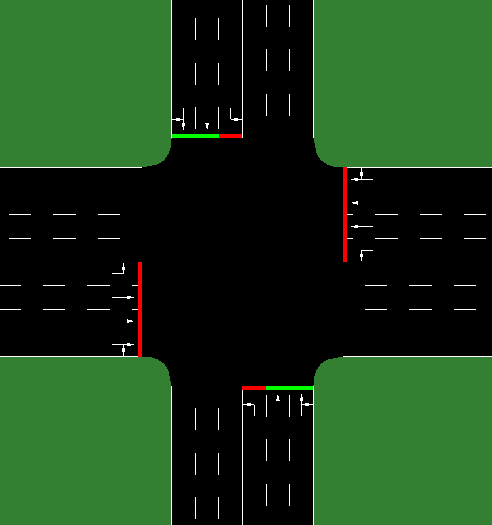
\includegraphics[width=0.5\columnwidth]{snap_envSUMO.png}}
    \caption{Snapshot of the traffic environment.}
    \label{fig:snap}
\end{figure}

\subsection{Methods and Current Implementation}

\subsubsection{Action space}

Different state-of-the-art algorithms have chosen different action space sizes, sometimes only dealing with 4 traffic light phases \cite{ref2}\cite{ref3} while others reach 8 \cite{ref1}\cite{ref4}. Defining a correct action space is important to allow an agent to choose an optimal action according to the current state. Consequently, the selected action space is the following: 1) North-South Straight (N-SS), 2) North-South Left (N-SL), 3) East-West Straight (E-WS), 4) East-West Left (E-WL), 5) East Straight and Left (ESL), 6) West Straight and Left (WSL), 7) South Straight and Left (SSL), and 8) North Straight and Left (NSL), right turns from the current green phases will be allowed in all states. These 8 possible actions will enable the agent to handle traffic jams originating from a single direction or multiple directions.

\subsubsection{Deep Reinforcement Learning Algorithms}

The two most common DRL approaches will be compared: Q-value methods and Policy Optimization Methods, to see which is better suited for this environment. The current implementation is located at the following \href{https://github.com/jazg97/TrafficSignalControl-RL}{GitHub repository}. Particularly, the following two methods will be compared:

\begin{itemize}
\item{Rainbow DQN}
\item{Proximal Policy Optimization}
\end{itemize}

As noted by \cite{ref3}, choosing a correct reward signal is fundamental for the agent to find an optimal policy, rewards such as queue length, average speed, total waiting time, or traffic volume are interesting options for the agent to receive.

\begin{thebibliography}{99}
\bibitem{ref1} L. Huang and X. Qu, “Improving traffic signal control operations using proximal policy optimization,” IET Intell. Transp. Syst., vol. 17, no. 3, pp. 592–605, 2023, doi: https://doi.org/10.1049/itr2.12286.
\bibitem{ref2} Y. Shi, Z. Wang, T. J. LaClair, C. Wang, Y. Shao, and J. Yuan, “A Novel Deep Reinforcement Learning Approach to Traffic Signal Control with Connected Vehicles †,” Appl. Sci., vol. 13, no. 4, 2023, doi: 10.3390/app13042750.
\bibitem{ref3} A. Fontoura, D. B. Haddad, and E. Bezerra, “A Deep Reinforcement Learning Approach to Adaptive Traffic Lights Management,” Proc. - 2019 Brazilian Conf. Intell. Syst. BRACIS 2019, no. Woa, pp. 216–221, 2019, doi: 10.1109/BRACIS.2019.00046.
\bibitem{ref4} H. Luo, Y. Bie, and S. Jin, “Reinforcement Learning for Traffic Signal Control in Hybrid Action Space,” IEEE Trans. Intell. Transp. Syst., vol. PP, pp. 1–17, 2024, doi: 10.1109/TITS.2023.3344585.
\end{thebibliography}

\end{document}
